\documentclass[border=3pt,tikz]{standalone}
\usepackage{amsmath}
\usetikzlibrary{calc}
\usetikzlibrary{arrows.meta} % for arrow size
\usetikzlibrary{calc}
\begin{document}
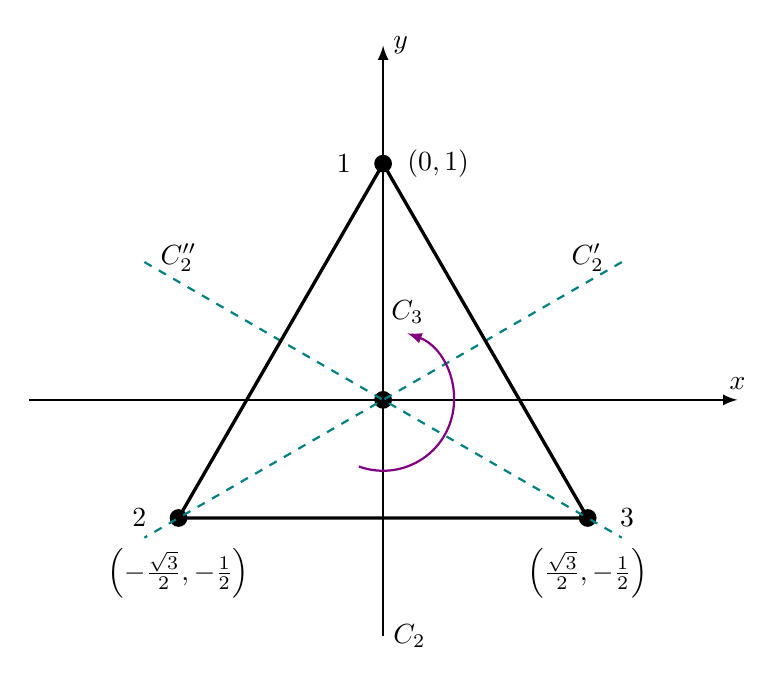
\begin{tikzpicture}[scale=3, extended line/.style={shorten >=-#1,shorten <=-#1},
    extended line/.default=1cm]
    
    \coordinate (P1) at (0, 1);
    \coordinate (P2) at ({-sqrt(3)/2}, -0.5);
    \coordinate (P3) at ({sqrt(3)/2}, -0.5);
    
    \filldraw[black] (0,0) circle (1pt);
    
    \node [xshift=-0.5cm] at(P1) {$1$};
    \filldraw[black] (P1) circle (1pt) node[xshift=0.7cm, scale=1] {$(0, 1)$};
    \filldraw[black] (P2) circle (1pt) node[yshift=-0.7cm, scale=1] {$\left(-\frac{\sqrt{3}}{2}, -\frac{1}{2}\right)$};
    \node [xshift=-0.5cm] at(P2) {$2$};

    \filldraw[black] (P3) circle (1pt) node[yshift=-0.7cm, scale=1] {$\left(\frac{\sqrt{3}}{2}, -\frac{1}{2}\right)$};
    \node [xshift=0.5cm] at(P3) {$3$};

    \draw[thick, -latex] (0, -1.) node [right] {$C_2$} -- (0, 1.5) node [right] {$y$};
    \draw[thick, -latex] (-1.5,0) -- (1.5, 0) node [above] {$x$};
    \draw[thick, teal, dashed, extended line=0.5cm] ({-sqrt(3)/2},  0.5)  node [above, black] {$C_2''$} -- (P3);
    \draw[thick, teal, dashed, extended line=0.5cm] ({sqrt(3)/2},  0.5)  node [above, black] {$C_2'$} -- (P2);
    \draw[very thick] (P1) -- (P2) -- (P3) -- (P1);

    \draw[violet, thick, -latex] ({0.3*cos(250)}, {0.3*sin(250)}) arc (-110:70:0.3);
    \node [above] at ({0.3*cos(70)}, {0.3*sin(70)}) {$C_3$};
    

    \end{tikzpicture}
\end{document}